%% LyX 2.2.2 created this file.  For more info, see http://www.lyx.org/.
%% Do not edit unless you really know what you are doing.
\documentclass[ruled]{article}
\usepackage{courier}
\usepackage[T1]{fontenc}
\usepackage[latin9]{inputenc}
\usepackage[letterpaper]{geometry}
\geometry{verbose}
\usepackage{color}
\usepackage{url}
\usepackage{algorithm2e}
\usepackage{amsmath}
\usepackage{amssymb}
\usepackage[unicode=true,
bookmarks=false,
breaklinks=false,pdfborder={0 0 1},backref=section,colorlinks=true]
{hyperref}
\usepackage{minted}
\makeatletter
\usepackage{graphicx}

%%%%%%%%%%%%%%%%%%%%%%%%%%%%%% LyX specific LaTeX commands.
\providecommand{\LyX}{\texorpdfstring%
	{L\kern-.1667em\lower.25em\hbox{Y}\kern-.125emX\@}
	{LyX}}

\@ifundefined{date}{}{\date{}}
%%%%%%%%%%%%%%%%%%%%%%%%%%%%%% User specified LaTeX commands.
\definecolor{mygreen}{rgb}{0,0.6,0}
\definecolor{mygray}{rgb}{0.5,0.5,0.5}
\definecolor{mymauve}{rgb}{0.58,0,0.82}

\makeatother

\usepackage{listings}
\lstset{backgroundcolor={\color{white}},
	basicstyle={\footnotesize\ttfamily},
	breakatwhitespace=false,
	breaklines=true,
	captionpos=b,
	commentstyle={\color{mygreen}},
	deletekeywords={...},
	escapeinside={\%*}{*)},
	extendedchars=true,
	frame=shadowbox,
	keepspaces=true,
	keywordstyle={\color{blue}},
	language=Python,
	morekeywords={*,...},
	numbers=none,
	numbersep=5pt,
	numberstyle={\tiny\color{mygray}},
	rulecolor={\color{black}},
	showspaces=false,
	showstringspaces=false,
	showtabs=false,
	stepnumber=1,
	stringstyle={\color{mymauve}},
	tabsize=2}
\begin{document}
	\global\long\def\reals{\mathbf{R}}
	\global\long\def\integers{\mathbf{Z}}
	\global\long\def\naturals{\mathbf{N}}
	\global\long\def\rationals{\mathbf{Q}}
	\global\long\def\ca{\mathcal{A}}
	\global\long\def\cb{\mathcal{B}}
	\global\long\def\cc{\mathcal{C}}
	\global\long\def\cd{\mathcal{D}}
	\global\long\def\ce{\mathcal{E}}
	\global\long\def\cf{\mathcal{F}}
	\global\long\def\cg{\mathcal{G}}
	\global\long\def\ch{\mathcal{H}}
	\global\long\def\ci{\mathcal{I}}
	\global\long\def\cj{\mathcal{J}}
	\global\long\def\ck{\mathcal{K}}
	\global\long\def\cl{\mathcal{L}}
	\global\long\def\cm{\mathcal{M}}
	\global\long\def\cn{\mathcal{N}}
	\global\long\def\co{\mathcal{O}}
	\global\long\def\cp{\mathcal{P}}
	\global\long\def\cq{\mathcal{Q}}
	\global\long\def\calr{\mathcal{R}}
	\global\long\def\cs{\mathcal{S}}
	\global\long\def\ct{\mathcal{T}}
	\global\long\def\cu{\mathcal{U}}
	\global\long\def\cv{\mathcal{V}}
	\global\long\def\cw{\mathcal{W}}
	\global\long\def\cx{\mathcal{X}}
	\global\long\def\cy{\mathcal{Y}}
	\global\long\def\cz{\mathcal{Z}}
	\global\long\def\ind#1{1(#1)}
	\global\long\def\pr{\mathbb{P}}
	
	\global\long\def\ex{\mathbb{E}}
	\global\long\def\var{\textrm{Var}}
	\global\long\def\cov{\textrm{Cov}}
	\global\long\def\sgn{\textrm{sgn}}
	\global\long\def\sign{\textrm{sign}}
	\global\long\def\kl{\textrm{KL}}
	\global\long\def\law{\mathcal{L}}
	\global\long\def\eps{\varepsilon}
	\global\long\def\convd{\stackrel{d}{\to}}
	\global\long\def\eqd{\stackrel{d}{=}}
	\global\long\def\del{\nabla}
	\global\long\def\loss{\ell}
	\global\long\def\tr{\operatorname{tr}}
	\global\long\def\trace{\operatorname{trace}}
	\global\long\def\diag{\text{diag}}
	\global\long\def\rank{\text{rank}}
	\global\long\def\linspan{\text{span}}
	\global\long\def\proj{\text{Proj}}
	\global\long\def\argmax{\operatornamewithlimits{arg\, max}}
	\global\long\def\argmin{\operatornamewithlimits{arg\, min}}
	\global\long\def\bfx{\mathbf{x}}
	\global\long\def\bfy{\mathbf{y}}
	\global\long\def\bfl{\mathbf{\lambda}}
	\global\long\def\bfm{\mathbf{\mu}}
	\global\long\def\calL{\mathcal{L}}
	\global\long\def\vw{\boldsymbol{w}}
	\global\long\def\vx{\boldsymbol{x}}
	\global\long\def\vxi{\boldsymbol{\xi}}
	\global\long\def\valpha{\boldsymbol{\alpha}}
	\global\long\def\vbeta{\boldsymbol{\beta}}
	\global\long\def\vsigma{\boldsymbol{\sigma}}
	\global\long\def\vmu{\boldsymbol{\mu}}
	\global\long\def\vtheta{\boldsymbol{\theta}}
	\global\long\def\vd{\boldsymbol{d}}
	\global\long\def\vs{\boldsymbol{s}}
	\global\long\def\vt{\boldsymbol{t}}
	\global\long\def\vh{\boldsymbol{h}}
	\global\long\def\ve{\boldsymbol{e}}
	\global\long\def\vf{\boldsymbol{f}}
	\global\long\def\vg{\boldsymbol{g}}
	\global\long\def\vz{\boldsymbol{z}}
	\global\long\def\vk{\boldsymbol{k}}
	\global\long\def\va{\boldsymbol{a}}
	\global\long\def\vb{\boldsymbol{b}}
	\global\long\def\vv{\boldsymbol{v}}
	\global\long\def\vy{\boldsymbol{y}}
	
	
	\title{Machine Learning and Computational Statistics\\
		\textbf{PRELIMINARY VERSION} Homework 5: Generalized Hinge Loss and
		Multiclass SVM}
	\author{Zhuoru Lin}
	
	
	\maketitle
	\textbf{Due: Thursday, April 6, 2017, at 10pm (Submit via Gradescope)}
	
	\textbf{Instructions}: Your answers to the questions below, including
	plots and mathematical work, should be submitted as a single PDF file.
	It's preferred that you write your answers using software that typesets
	mathematics (e.g. \LaTeX{}, \LyX{}, or MathJax via iPython), though
	if you need to you may scan handwritten work. You may find the \href{https://github.com/gpoore/minted}{minted}
	package convenient for including source code in your \LaTeX{} document.
	If you are using \LyX{}, then the \href{https://en.wikibooks.org/wiki/LaTeX/Source_Code_Listings}{listings}
	package tends to work better.
	
	
	\section{Introduction}
	
	\textbf{NOTE: THIS PROBLEM SET IS NOT YET COMPLETE. A SIGNIFICANT
		PROGRAMMING PORTION WILL SOON BE ADDED. STAY TUNED.}
	
	The goal of this problem set is to get more comfortable with the multiclass
	hinge loss and multiclass SVM. In several problems below, you are
	asked to justify that certain functions are convex. For these problems,
	you may use any of the rules about convex functions described in our
	notes on Convex Optimization (\url{https://davidrosenberg.github.io/mlcourse/Notes/convex-optimization.pdf})
	or in the Boyd and Vandenberghe book. In particular, you will need
	to make frequent use of the following result: If $f_{1},\ldots,f_{m}:\reals^{n}\to\reals$
	are convex, then their pointwise maximum
	\[
	f(x)=\max\left\{ f_{1}(x),\ldots,f_{m}(x)\right\} 
	\]
	is also convex. 
	\pagebreak
	
	\section{Convex Surrogate Loss Functions}
	
	It's common in machine learning that the loss functions we really
	care about lead to optimization problems that are not computationally
	tractable. The $0/1$ loss for binary classification is one such example\footnote{Interestingly, if our hypothesis space is linear classifiers and we
		are in the ``realizable'' case, which means that there is some hypothesis
		that achieves $0$ loss (with the 0/1 loss), then we can efficiently
		find a good hypothesis using linear programming. This is not difficult
		to see: each data point gives a single linear constraint, and we are
		looking for a vector that satisfies the constraints for each data
		point.}. Since we have better machinery for minimizing convex functions,
	a standard approach is to find a \textbf{convex surrogate loss function.
	}A convex surrogate loss function is a convex function that is an
	upper bound for the loss function of interest\footnote{At this level of generality, you might be wondering: ``A convex function
		of WHAT?''. For binary classification, we usually are talking about
		a convex function of the margin. But to solve our machine learning
		optimization problems, we will eventually need our loss function to
		be a convex function of some $w\in\reals^{d}$ that parameterizes
		our hypothesis space. It'll be clear in what follows what we're talking
		about.}. If we can make the upper bound small, then the loss we care about
	will also be small\footnote{This is actually fairly weak motivation for a convex surrogate. Much
		better motivation comes from the more advanced theory of \textbf{classification
			calibrated} loss functions. See Bartlett et al's paper ``Convexity,
		Classification, and Risk Bounds.'' \url{http://www.eecs.berkeley.edu/~wainwrig/stat241b/bartlettetal.pdf}}. Below we will show that the multiclass hinge loss based on a class-sensitive
	loss $\Delta$ is a convex surrogate for the multiclass loss function
	$\Delta$, when we have a linear hypothesis space. We'll start with
	a special case, that the hinge loss is a convex surrogate for the
	$0/1$ loss.
	\pagebreak
	
	%%%%%%%%%%%%%%%%%%%%%%%%%%%%%%%%%%%%%%%%%%%%%%%%%%%%%%%%
	%%%%%%%%%%%%%%%%%%%%%%%%%%%%%%%%%%%%%%%%%%%%%%%%%%%%%%%%
	%%%%%%%%%%%%%%%%%%%%%%%%%%%%%%%%%%%%%%%%%%%%%%%%%%%%%%%%
	%2.1 
	%%%%%%%%%%%%%%%%%%%%%%%%%%%%%%%%%%%%%%%%%%%%%%%%%%%%%%%%%%%%%%%%%%%%%%%%%%%%%%%%%%%%%%%%%%%%%%%%%%%%%%%%%%%%%%%%%%%%%%%%%%%%%%%%%%%%%%%%%%%%%%%%%%%%%%%%%%%%%%%%%%%%%%%%%%%%%%%%%%%%%%%%%%%%%%%%%%%%%%%%%%%%%%%%%%%%%%%%%%%%%%%%
	\subsection{Hinge loss is a convex surrogate for 0/1 loss}
	\begin{enumerate}
		\item Let $f:\cx\to\reals$ be a classification score function for binary
		classification. 
		\begin{enumerate}
			\item For any example $(x,y)\in\cx\times\left\{ -1,1\right\} $, show that
			\[
			\ind{y\neq\sign(f(x)}\le\max\left\{ 0,1-yf(x)\right\} ,
			\]
			where $\sign\left(x\right)=\begin{cases}
			1 & x>0\\
			0 & x=0\\
			-1 & x<0
			\end{cases}$.
			\\
			\noindent\rule{16cm}{2pt}
			\\
			%%%%%%%%%%%%%%%%%%%%%%%%%%%%%%%%%%%%%%%%%%%%%%%%%%%%%%%%
			%2.1.A Answer
			%%%%%%%%%%%%%%%%%%%%%%%%%%%%%%%%%%%%%%%%%%%%%%%%%%%%%%%%
			Answers: If $y=sign(x)$. Then $yf(x)>0$. We automatically have $1(y \neq sign(f(x)))=0\leq max(0,1-yf(x))$. \\
			\\
			If $y \neq sign(f(x))$, then $yf(x)<0$ and $1=1(y \neq sign(f(x))) \leq 1-yf(x)=max(0,1-yf(x))$.
			\item Show that the hinge loss $\max\left\{ 0,1-m\right\} $ is a convex
			function of the margin $m$.
			\\
			
			Answer: Since both 0 and 1-m are convex function of m. $max(0,1-m)$
			
			\item Suppose our prediction score functions are given by $f_{w}(x)=w^{T}x$.
			The hinge loss of $f_{w}$ on any example $\left(x,y\right)$ is then
			$\max\left\{ 0,1-yw^{T}x\right\} $. Show that this is a convex function
			of $w$. 
			
			Define $g(w)=1-yw^Tx$ and $g'(w')=1-y-w'^Tx$. Then we have:
			
			\begin{align*}
			g(\theta w+(1-\theta)w')&=1-y(\theta w+(1-\theta)yw't)^Tx\\
			&=1-\theta yw^Tx -(1-\theta)yw'^Tx\\
			&\leq (1-\theta yw^Tx)+(1 -(1-\theta)yw'^Tx)\\
			&=g(\theta w)+g((1-\theta)w').
			\end{align*}
			Hence $g(w)$ is a convex function, so is $max\{0,g(w)\}$.
			
		\end{enumerate}
	\end{enumerate}
	
	%%%%%%%%%%%%%%%%%%%%%%%%%%%%%%%%%%%%%%%%%%%%%%%%%%%%%%%%%%%%%%%%%%%%%%%%%%%%%%%%%%%%%%%%%%%%%%%%%%%%%%%%%%%%%%%%
	%2.2
	%%%%%%%%%%%%%%%%%%%%%%%%%%%%%%%%%%%%%%%%%%%%%%%%%%%%%%%%%%%%%%%%%%%%%%%%%%%%%%%%%%%%%%%%%%%%%%%%%%%%%%%%%%%%%%%%
	\pagebreak
	\subsection{Generalized Hinge Loss}
	
	Consider the multiclass output space $\cy=\left\{ 1,\ldots,k\right\} $.
	Suppose we have a base hypothesis space \textbf{$\ch=\left\{ h:\cx\times\cy\to\reals\right\} $
	}from which we select a compatibility score function. Then our final
	multiclass hypothesis space is $\cf=\left\{ f(x)=\argmax_{y\in\cy}h(x,y)\mid h\in\ch\right\} $.
	Since functions in $\cf$ map into $\cy$, our action space $\ca$
	and output space $\cy$ are the same. Nevertheless, we will write
	our class-sensitive loss function as $\Delta:\cy\times\ca\to\reals$,
	even though $\cy=\ca$. We do this to indicate that the true class
	goes in the first slot of the function, while the prediction (i.e.
	the action) goes in the second slot. This is important because we
	do not assume that $\Delta(y,y')=\Delta(y',y)$. It would not be unusual
	to have this asymmetry in practice. For example, false alarms may
	be much less costly than no alarm when indeed something is going wrong.
	
	Our ultimate goal would be to find $f\in\cf$ minimizing the empirical
	cost-sensitive loss:
	\[
	\min_{f\in\cf}\sum_{i=1}^{n}\Delta\left(y_{i},f(x_{i})\right).
	\]
	Since binary classification with $0/1$ loss is both intractable and
	a special case of this formulation, we know that this more general
	formulation must also be computationally intractable. Thus we are
	looking for a convex surrogate loss function.
	%%%%%%%%%%%%%%%%%%%%%%%%%%%%%%%%%%%%%%%%%%%%%%%%%%%%%%%%
	%2.2.1
	%%%%%%%%%%%%%%%%%%%%%%%%%%%%%%%%%%%%%%%%%%%%%%%%%%%%%%%%
	\begin{enumerate}
		\item Suppose we have chosen an $h\in\ch$, from which we get the decision
		function $f(x)=\argmax_{y\in\cy}h(x,y)$. Justify that for any $x\in\cx$
		and $y\in\cy$, we have 
		\[
		h(x,y)\le h(x,f(x)).
		\]
		\\
		\noindent\rule{16cm}{2pt}
		%%%%%%%%%%%%%%%%%%%%%%%%%%%%%%%%%%%%%%%%%%%%%%%%%%%%%%%%
		%2.2.1 Answer
		%%%%%%%%%%%%%%%%%%%%%%%%%%%%%%%%%%%%%%%%%%%%%%%%%%%%%%%%
		Answer: f(x) is define to be the $y \in \cy$ such that h(x,y) is at maximun. We automatically have $h(x,y)\le h(x,f(x))$ for all x.
		
		\pagebreak
		
		%%%%%%%%%%%%%%%%%%%%%%%%%%%%%%%%%%%%%%%%%%%%%%%%%%%%%%%%
		%2.2.2
		%%%%%%%%%%%%%%%%%%%%%%%%%%%%%%%%%%%%%%%%%%%%%%%%%%%%%%%%
		\item Justify the following two inequalities:
		\begin{eqnarray*}
			\Delta\left(y,f(x)\right) & \le & \Delta\left(y,f(x)\right)+h(x,f(x))-h(x,y)\\
			& \le & \max_{y'\in\cy}\left[\Delta\left(y,y')\right)+h(x,y')-h(x,y)\right]
		\end{eqnarray*}
		The RHS of the last expression is called the \textbf{generalized hinge
			loss:}
		\[
		\ell\left(h,\left(x,y\right)\right)=\max_{y'\in\cy}\left[\Delta\left(y,y')\right)+h(x,y')-h(x,y)\right].
		\]
		We have shown that for any $x\in\cx,y\in\cy,h\in\ch$ we have
		\[
		\ell\left(h,(x,y)\right)\ge\Delta(y,f(x)),
		\]
		where, as usual, $f(x)=\argmax_{y\in\cy}h(x,y)$. {[}You should think
		about why we cannot write the generalized hinge loss as $\ell\left(f,(x,y)\right)$.{]}
		\\
		\noindent\rule{16cm}{2pt}
		%%%%%%%%%%%%%%%%%%%%%%%%%%%%%%%%%%%%%%%%%%%%%%%%%%%%%%%%
		%2.2.2 Answer
		%%%%%%%%%%%%%%%%%%%%%%%%%%%%%%%%%%%%%%%%%%%%%%%%%%%%%%%%
		Answer: Since $f(x)=argmax_{y\in\cy}h(x,y)$ , we must have $h(x,f(x))\le h(x,y)$. Therefore: $\Delta\left(y,f(x)\right) \le\Delta\left(y,f(x)\right)+h(x,f(x))-h(x,y).$  Since $f(x) \in \ca$, we automatically have the second inequality.
		\pagebreak
		
		%%%%%%%%%%%%%%%%%%%%%%%%%%%%%%%%%%%%%%%%%%%%%%%%%%%%%%%%
		%2.2.3
		%%%%%%%%%%%%%%%%%%%%%%%%%%%%%%%%%%%%%%%%%%%%%%%%%%%%%%%%
		\item We now introduce a specific base hypothesis space $\ch$ of linear
		functions. Consider a class-sensitive feature mapping $\Psi:\cx\times\cy\to\reals^{d}$,
		and $\ch=\left\{ h_{w}\left(x,y\right)=\left\langle w,\Psi(x,y)\right\rangle \mid w\in\reals^{d}\right\} $.
		Show that we can write the generalized hinge loss for $h_{w}(x,y)$
		on example $\left(x_{i},y_{i}\right)$ as
		\[
		\ell\left(h_{w},(x_{i},y_{i})\right)=\max_{y\in\cy}\left[\Delta\left(y_{i},y)\right)+\left\langle w,\Psi(x_{i},y)-\Psi(x_{i},y_{i})\right\rangle \right].
		\]
		\\
		\noindent\rule{16cm}{2pt}
		%%%%%%%%%%%%%%%%%%%%%%%%%%%%%%%%%%%%%%%%%%%%%%%%%%%%%%%%
		%2.2.3 Answer
		%%%%%%%%%%%%%%%%%%%%%%%%%%%%%%%%%%%%%%%%%%%%%%%%%%%%%%%%
		Answer: By definition of generalized hinge loss from part 2, we have:
		\begin{align*}
		\ell \left(h_w,(x_i,y_i)\right)&=\max_{y\in\cy}\left[\Delta(y_i,y)+h(x_i,y)-h(x_i,y_i) \right]\\
		&=\max_{y\in\cy}\left[\Delta\left(y_{i},y)\right)+\left\langle w,\Psi(x_{i},y)-\Psi(x_{i},y_{i})\right\rangle \right].
		\end{align*}
		
		
		%%%%%%%%%%%%%%%%%%%%%%%%%%%%%%%%%%%%%%%%%%%%%%%%%%%%%%%%
		%2.1.4
		%%%%%%%%%%%%%%%%%%%%%%%%%%%%%%%%%%%%%%%%%%%%%%%%%%%%%%%%
		\pagebreak
		\item We will now show that the generalized hinge loss $\ell\left(h_{w},(x_{i},y_{i})\right)$
		is a convex function of $w$. Justify each of the following steps.
		\begin{enumerate}
			\item The expression $\Delta(y_{i},y)+\left\langle w,\Psi(x_{i},y)-\Psi(x_{i},y_{i})\right\rangle $
			is an affine function of $w$.
			\item The expression $\max_{y\in\cy}\left[\Delta\left(y_{i},y)\right)+\left\langle w,\Psi(x_{i},y)-\Psi(x_{i},y_{i})\right\rangle \right]$
			is a convex function of $w$. 
		\end{enumerate}
		\noindent\rule{16cm}{2pt}
		%%%%%%%%%%%%%%%%%%%%%%%%%%%%%%%%%%%%%%%%%%%%%%%%%%%%%%%%
		%2.2.4 Answer
		%%%%%%%%%%%%%%%%%%%%%%%%%%%%%%%%%%%%%%%%%%%%%%%%%%%%%%%%
		Answer: \\
		(a) $\Delta(y_{i},y)+\left\langle w,\Psi(x_{i},y)-\Psi(x_{i},y_{i})\right\rangle=\Delta(y_{i},y)+w^T(\Psi(x_i,y)-\Psi(x_i,y_i))$ is an affine function of $w$.\\
		(b) By part (a) $\Delta(y_{i},y)+\left\langle w,\Psi(x_{i},y)-\Psi(x_{i},y_{i})\right\rangle$ is an affine function of $w$, therefore is also a convex function of $w$. $\max_{y\in\cy}\left[\Delta\left(y_{i},y)\right)+\left\langle w,\Psi(x_{i},y)-\Psi(x_{i},y_{i})\right\rangle \right]$ is the pointwise maximun of a group of convex function, hence is also a convex function of $w$.
		%%%%%%%%%%%%%%%%%%%%%%%%%%%%%%%%%%%%%%%%%%%%%%%%%%%%%%%%
		%2.5
		%%%%%%%%%%%%%%%%%%%%%%%%%%%%%%%%%%%%%%%%%%%%%%%%%%%%%%%%
		\pagebreak
		\item Conclude that $\ell\left(h_{w},(x_{i},y_{i})\right)$ is a convex
		surrogate for $\Delta(y_{i},f_{w}(x_{i}))$.
	\end{enumerate}
	\noindent\rule{16cm}{2pt}
	%%%%%%%%%%%%%%%%%%%%%%%%%%%%%%%%%%%%%%%%%%%%%%%%%%%%%%%%
	%2.5 answer
	%%%%%%%%%%%%%%%%%%%%%%%%%%%%%%%%%%%%%%%%%%%%%%%%%%%%%%%%
	Answer: By part 2, we know that $\ell\left(h_{w},(x_{i},y_{i})\right)$  is a surrogate for  $\Delta(y_{i},f_{w}(x_{i}))$. By part 4 we know $\ell\left(h_{w},(x_{i},y_{i})\right)$  is convex. There fore $\ell\left(h_{w},(x_{i},y_{i})\right)$  is a convex surrogate of $\Delta(y_{i},f_{w}(x_{i}))$.
	
	
	%%%%%%%%%%%%%%%%%%%%%%%%%%%%%%%%%%%%%%%%%%%%%%%%%%%%%%%%
	%%%%%%%%%%%%%%%%%%%%%%%%%%%%%%%%%%%%%%%%%%%%%%%%%%%%%%%%
	%3 SGD for Multiclass SVM
	%%%%%%%%%%%%%%%%%%%%%%%%%%%%%%%%%%%%%%%%%%%%%%%%%%%%%%%%
	%%%%%%%%%%%%%%%%%%%%%%%%%%%%%%%%%%%%%%%%%%%%%%%%%%%%%%%%
	\pagebreak
	\section{SGD for Multiclass SVM}
	
	Suppose our output space and our action space are given as follows:
	$\cy=\ca=\left\{ 1,\ldots,k\right\} $. Given a non-negative class-sensitive
	loss function $\Delta:\cy\times\ca\to\reals^{\ge0}$ and a class-sensitive
	feature mapping $\Psi:\cx\times\cy\to\reals^{d}$. Our prediction
	function $f:\cx\to\cy$ is given by
	\[
	f_{w}(x)=\argmax_{y\in\cy}\left\langle w,\Psi(x,y)\right\rangle 
	\]
	
	\begin{enumerate}
		%%%%%%%%%%%%%%%%%%%%%%%%%%%%%%%%%%%%%%%%%%%%%%%%%%%%%%%%
		%3.1
		%%%%%%%%%%%%%%%%%%%%%%%%%%%%%%%%%%%%%%%%%%%%%%%%%%%%%%%%
		\item For a training set $(x_{1},y_{1}),\ldots(x_{n},y_{n})$, let $J(w)$
		be the $\ell_{2}$-regularized empirical risk function for the multiclass
		hinge loss. We can write this as
		\[
		J(w)=\lambda\|w\|^{2}+\frac{1}{n}\sum_{i=1}^{n}\max_{y\in\cy}\left[\Delta\left(y_{i},y\right)+\left\langle w,\Psi(x_{i},y)-\Psi(x_{i},y_{i})\right\rangle \right].
		\]
		We will now show that $J(w)$ is a convex function of $w$. Justify
		each of the following steps. As we've shown it in a previous problem,
		you may use the fact that $w\mapsto\max_{y\in\cy}\left[\Delta\left(y_{i},y\right)+\left\langle w,\Psi(x_{i},y)-\Psi(x_{i},y_{i})\right\rangle \right]$
		is a convex function.
		\begin{enumerate}
			\item $\frac{1}{n}\sum_{i=1}^{n}\max_{y\in\cy}\left[\Delta\left(y_{i},y\right)+\left\langle w,\Psi(x_{i},y)-\Psi(x_{i},y_{i})\right\rangle \right]$
			is a convex function of $w$.
			\item $\|w\|^{2}$ is a convex function of $w$.
			\item $J(w)$ is a convex function of $w$.
		\end{enumerate}
		\noindent\rule{16cm}{2pt}
		%%%%%%%%%%%%%%%%%%%%%%%%%%%%%%%%%%%%%%%%%%%%%%%%%%%%%%%%
		%3.1 Answer
		%%%%%%%%%%%%%%%%%%%%%%%%%%%%%%%%%%%%%%%%%%%%%%%%%%%%%%%%
		Answer:\\
		(a) Since $w\mapsto\max_{y\in\cy}\left[\Delta\left(y_{i},y\right)+\left\langle w,\Psi(x_{i},y)-\Psi(x_{i},y_{i})\right\rangle \right]$ is a convex function. The summation of convex functions is convex. Thus $\frac{1}{n}\sum_{i=1}^{n}\max_{y\in\cy}\left[\Delta\left(y_{i},y\right)+\left\langle w,\Psi(x_{i},y)-\Psi(x_{i},y_{i})\right\rangle \right]$ is a convex function of $w$.\\
		(b) Since $\|w\|$ is a convex function of $w$. Then $\|w\|^{2}$ is a composition of convex function, which is convex.\\
		(c) By part (a) and (b) we have $J(w)$ is a summation of convex function, which is convex. 
		
		%%%%%%%%%%%%%%%%%%%%%%%%%%%%%%%%%%%%%%%%%%%%%%%%%%%%%%%%
		%3.2
		%%%%%%%%%%%%%%%%%%%%%%%%%%%%%%%%%%%%%%%%%%%%%%%%%%%%%%%%
		\pagebreak
		\item Since $J(w)$ is convex, it has a subgradient at every point. Give
		an expression for a subgradient of $J(w)$. You may use any standard
		results about subgradients, including the result from an earlier homework
		about subgradients of the pointwise maxima of functions. (Hint: It
		may be helpful to refer to $\hat{y}_{i}=\argmax_{y\in\cy}\left[\Delta\left(y_{i},y\right)+\left\langle w,\Psi(x_{i},y)-\Psi(x_{i},y_{i})\right\rangle \right]$.)
		\noindent\rule{16cm}{2pt}
		%%%%%%%%%%%%%%%%%%%%%%%%%%%%%%%%%%%%%%%%%%%%%%%%%%%%%%%%
		%3.2 Answer
		%%%%%%%%%%%%%%%%%%%%%%%%%%%%%%%%%%%%%%%%%%%%%%%%%%%%%%%%
		Answer: \\
		Let $\hat{y}_{i}=\argmax_{y\in\cy}\left[\Delta\left(y_{i},y\right)+\left\langle w,\Psi(x_{i},y)-\Psi(x_{i},y_{i})\right\rangle \right]$.\\
		Claim: $g(w) = 2 \lambda w^T+\frac{1}{n}\sum \limits_{i=1}^n\left[ (\Psi(x,\hat{y}_{i})-\Psi(x,y_i))\right]$ is a subgradient of $J(w)$.\\
		Proof: 
		
		\begin{align*}
		J(w+v) &= \lambda \|w+v\|^2+\frac{1}{n}\sum \limits_{i=1}^n \max_{y\in\cy}\left[\Delta\left(y_{i},y\right)+\left\langle w+v,\Psi(x_{i},y)-\Psi(x_{i},y_{i})\right\rangle \right]\\
		&\geq \lambda \|w\|^2+\lambda\|v\|^2+2\lambda w^Tv+\frac{1}{n}\sum \limits_{i=1}^n \left[\Delta\left(y_{i},\hat{y}_{i}\right)+\left\langle w,\Psi(x_{i},\hat{y}_{i})-\Psi(x_{i},y_{i})\right\rangle\right] \\
		&+\frac{1}{n}\left[\sum \limits_{i=1}^n \left\langle v,\Psi(x_{i},\hat{y}_{i})-\Psi(x_{i},y_{i})\right\rangle \right]\\
		&=J(w)+gv+\lambda \|v\|^2\\
		&\geq J(w)+gv
		\end{align*}
		
		%%%%%%%%%%%%%%%%%%%%%%%%%%%%%%%%%%%%%%%%%%%%%%%%%%%%%%%%
		%3.3
		%%%%%%%%%%%%%%%%%%%%%%%%%%%%%%%%%%%%%%%%%%%%%%%%%%%%%%%%
		\pagebreak
		\item Give an expression the stochastic subgradient based on the point $(x_{i},y_{i})$.\\
		\noindent\rule{16cm}{2pt}
		\\
		%%%%%%%%%%%%%%%%%%%%%%%%%%%%%%%%%%%%%%%%%%%%%%%%%%%%%%%%
		%3.3 Answer
		%%%%%%%%%%%%%%%%%%%%%%%%%%%%%%%%%%%%%%%%%%%%%%%%%%%%%%%%
		Answer: $2 \lambda w^T+\left[ (\Psi(x_{i},\hat{y_{i}})-\Psi(x,y_i))\right]$
		%%%%%%%%%%%%%%%%%%%%%%%%%%%%%%%%%%%%%%%%%%%%%%%%%%%%%%%%
		%3.4
		%%%%%%%%%%%%%%%%%%%%%%%%%%%%%%%%%%%%%%%%%%%%%%%%%%%%%%%%
		\pagebreak
		\item Give an expression for a minibatch subgradient, based on the points
		$(x_{i},y_{i}),\ldots,\left(x_{i+m-1},y_{i+m-1}\right)$. 
	\end{enumerate}
	\noindent\rule{16cm}{2pt}\\
	%%%%%%%%%%%%%%%%%%%%%%%%%%%%%%%%%%%%%%%%%%%%%%%%%%%%%%%%
	%3.4 Answer
	%%%%%%%%%%%%%%%%%%%%%%%%%%%%%%%%%%%%%%%%%%%%%%%%%%%%%%%%
	Answer: $2 \lambda w^T+\frac{1}{m}\sum \limits_{i}^{i+m-1}\left[ (\Psi(x_{i},\hat{y_{i}})-\Psi(x,y_i))\right]$
	
	
	
	
	
	
	
	%%%%%%%%%%%%%%%%%%%%%%%%%%%%%%%%%%%%%%%%%%%%%%%%%%%%%%%%
	%%%%%%%%%%%%%%%%%%%%%%%%%%%%%%%%%%%%%%%%%%%%%%%%%%%%%%%%
	%4 Optional
	%%%%%%%%%%%%%%%%%%%%%%%%%%%%%%%%%%%%%%%%%%%%%%%%%%%%%%%%
	%%%%%%%%%%%%%%%%%%%%%%%%%%%%%%%%%%%%%%%%%%%%%%%%%%%%%%%%
	\pagebreak
	\section{{[}OPTIONAL{]} Another Formulation of Generalized Hinge Loss}
	
	In lecture we defined the \textbf{margin} of the compatibility score
	function $h$ on the $i$th example $(x_{i},y_{i})$ for class $y$
	as
	\[
	m_{i,y}(h)=h(x_{i},y_{i})-h(x_{i},y),
	\]
	and the loss on an individual example $\left(x_{i},y_{i}\right)$
	to be:
	
	\[
	\max_{y}\left(\left[\Delta(y_{i},y)-m_{i,y}(h)\right]_{+}\right).
	\]
	Here we investigate whether this is just an instance of the generalized
	hinge loss $\ell\left(h,\left(x,y\right)\right)$ defined above.
	\begin{enumerate}
		%%%%%%%%%%%%%%%%%%%%%%%%%%%%%%%%%%%%%%%%%%%%%%%%%%%%%%%%
		%4.1
		%%%%%%%%%%%%%%%%%%%%%%%%%%%%%%%%%%%%%%%%%%%%%%%%%%%%%%%%
		\item Show that $\ell\left(h,\left(x_{i},y_{i}\right)\right)=\max_{y'\in\cy}\left[\Delta\left(y_{i},y'\right)-m_{i,y'}(h)\right]$.
		(In other words, it looks just like loss above, but without the positive
		part.) 
		\\
		\noindent\rule{16cm}{2pt}
		%%%%%%%%%%%%%%%%%%%%%%%%%%%%%%%%%%%%%%%%%%%%%%%%%%%%%%%%
		%4.1 Answer
		%%%%%%%%%%%%%%%%%%%%%%%%%%%%%%%%%%%%%%%%%%%%%%%%%%%%%%%%
		Answer: \\
		By part 2.2.2, according to the definition of generalized hinge loss:\\
		\begin{align*}
		\ell\left(h,\left(x_{i},y_{i}\right)\right)&=\max_{y'\in\cy}\left[\Delta\left(y_{i},y'\right)+h(x_{i},y')-h(x_i,y_{i})\right]\\
		&=\max_{y'\in\cy}\left[\Delta\left(y_{i},y'\right)-m_{i,y'}(h)\right]
		\end{align*}
		
		%%%%%%%%%%%%%%%%%%%%%%%%%%%%%%%%%%%%%%%%%%%%%%%%%%%%%%%%
		%4.2
		%%%%%%%%%%%%%%%%%%%%%%%%%%%%%%%%%%%%%%%%%%%%%%%%%%%%%%%%
		\pagebreak
		\item Suppose $\Delta\left(y,y'\right)\ge0$ for all $y,y'\in\cy$. Show
		that for any example $\left(x_{i},y_{i}\right)$ and any score function
		$h$, the multiclass hinge loss we gave in lecture and the generalized
		hinge loss presented above are equivalent, in the sense that
		\[
		\max_{y\in\cy}\left(\left[\Delta(y_{i},y)-m_{i,y}(h)\right]_{+}\right)=\max_{y\in\cy}\left(\Delta(y_{i},y)-m_{i,y}(h)\right).
		\]
		(Hint: This is easy by piecing together other results we have already
		attained regarding the relationship between $\ell$ and $\Delta$.)
		\\
		\noindent\rule{16cm}{2pt}
		%%%%%%%%%%%%%%%%%%%%%%%%%%%%%%%%%%%%%%%%%%%%%%%%%%%%%%%%
		%4.2 Answer
		%%%%%%%%%%%%%%%%%%%%%%%%%%%%%%%%%%%%%%%%%%%%%%%%%%%%%%%%
		Answer: By conclusion of part 2.2.2, we have: $\ell\left(h,(x,y)\right)=\max_{y\in\cy}\left(\Delta(y_{i},y)-m_{i,y}(h)\right)\geq \Delta(y,f(x))\geq 0$. Hence $\max_{y\in\cy}\left(\Delta(y_{i},y)-m_{i,y}(h)\right)$ is non-negative, therefore:\\
		\[
		\max_{y\in\cy}\left(\left[\Delta(y_{i},y)-m_{i,y}(h)\right]_{+}\right)=\max_{y\in\cy}\left(\Delta(y_{i},y)-m_{i,y}(h)\right).
		\]
		
		%%%%%%%%%%%%%%%%%%%%%%%%%%%%%%%%%%%%%%%%%%%%%%%%%%%%%%%%
		%4.3
		%%%%%%%%%%%%%%%%%%%%%%%%%%%%%%%%%%%%%%%%%%%%%%%%%%%%%%%%
		\pagebreak
		\item In the context of the generalized hinge loss, $\Delta(y,y')$ is like
		the ``target margin'' between the score for true class $y$ and
		the score for class $y'$. Suppose that our prediction function $f$
		gets the correct class on $x_{i}$. That is, $f(x_{i})=\argmax_{y'\in\cy}h(x_{i},y')=y_{i}$.
		Furthermore, assume that all of our target margins are reached or
		exceeded. That is
		\[
		m_{i,y}(h)=h(x_{i},y_{i})-h(x_{i},y)\ge\Delta(y_{i},y),
		\]
		for all $y\neq y_{i}$. It seems like in this case, we should have
		$0$ loss. This is almost the case. Show that $\ell\left(h,(x_{i},y_{i})\right)=0$
		if we assume that $\Delta\left(y,y\right)=0$ for all $y\in\cy$. 
	\end{enumerate}
	\noindent\rule{16cm}{2pt}
	%%%%%%%%%%%%%%%%%%%%%%%%%%%%%%%%%%%%%%%%%%%%%%%%%%%%%%%%
	%4.3 Answer
	%%%%%%%%%%%%%%%%%%%%%%%%%%%%%%%%%%%%%%%%%%%%%%%%%%%%%%%%
	Answer:  Since $m_{i,y}(h)=h(x_{i},y_{i})-h(x_{i},y)\ge\Delta(y_{i},y)$, then $\ell\left(h,(x_{i},y_{i})\right)=\Delta(y_{i},y)-m_{i,y}(h) \le 0$. Also by conclusion of 2.2.2 we also have $\ell\left(h,(x_{i},y_{i})\right) \geq \Delta(y_{i},f(x))=\Delta(y_{i},y_{i})\geq 0$. Therefore $\ell\left(h,(x_{i},y_{i})\right)=0$.
	
	%%%%%%%%%%%%%%%%%%%%%%%%%%%%%%%%%%%%%%%%%%%%%%%%%%%%%%%%
	%%%%%%%%%%%%%%%%%%%%%%%%%%%%%%%%%%%%%%%%%%%%%%%%%%%%%%%%
	% 5 Optional
	%%%%%%%%%%%%%%%%%%%%%%%%%%%%%%%%%%%%%%%%%%%%%%%%%%%%%%%%
	%%%%%%%%%%%%%%%%%%%%%%%%%%%%%%%%%%%%%%%%%%%%%%%%%%%%%%%%
	\pagebreak
	\section{{[}OPTIONAL{]} Hinge Loss is a Special Case of Generalized Hinge
		Loss}
	Let $\cy=\left\{ -1,1\right\} $. Let $\Delta(y,\hat{y})=\ind{y\neq\hat{y}}.$
	If $g(x)$ is the score function in our binary classification setting,
	then define our compatibility function as 
	\begin{eqnarray*}
		h(x,1) & = & g(x)/2\\
		h(x,-1) & = & -g(x)/2.
	\end{eqnarray*}
	Show that for this choice of $h$, the multiclass hinge loss reduces
	to hinge loss: 
	\[
	\ell\left(h,\left(x,y\right)\right)=\max_{y'\in\cy}\left[\Delta\left(y,y')\right)+h(x,y')-h(x,y)\right]=\max\left\{ 0,1-yg(x)\right\} 
	\]
	\noindent\rule{16cm}{2pt}
	%%%%%%%%%%%%%%%%%%%%%%%%%%%%%%%%%%%%%%%%%%%%%%%%%%%%%%%%
	%5 Answer
	%%%%%%%%%%%%%%%%%%%%%%%%%%%%%%%%%%%%%%%%%%%%%%%%%%%%%%%%
	Answer: generally there exist only two cases of $\Delta\left(y,y')\right)+h(x,y')-h(x,y)$\\
	If $y'=y$ we have $h\left(x,y'\right)-h\left(x,y\right)=0$ and $\Delta\left(y,y'\right)=0$. Therefore: $\Delta\left(y,y')\right)+h(x,y')-h(x,y)=0$.\\
	\\
	If $y'\neq y$, it can be computed that for both cases of $y=1$ and $y=-1$, $\Delta\left(y,y')\right)+h(x,y')-h(x,y)=1-yg(x)$.\\
	\\
	Hence $\ell\left(h,\left(x,y\right)\right)=\max_{y'\in\cy}\left[\Delta\left(y,y')\right)+h(x,y')-h(x,y)\right]=\max\left\{ 0,1-yg(x)\right\} $.
	
	%%%%%%%%%%%%%%%%%%%%%%%%%%%%%%%%%%%%%%%%%%%%%%%%%%%%%%%%
	%6 
	%%%%%%%%%%%%%%%%%%%%%%%%%%%%%%%%%%%%%%%%%%%%%%%%%%%%%%%%
	\pagebreak
	\section{Multiclass Classification - Implementation}
	
	In this problem we will work on a simple three-class classification
	example, similar to the one \href{https://davidrosenberg.github.io/mlcourse/Archive/2016/Lectures/9a.multiclass.pdf\#page=10}{given in lecture}.
	The data is generated and plotted for you in the skeleton code. 
	
	
	%%%%%%%%%%%%%%%%%%%%%%%%%%%%%%%%%%%%%%%%%%%%%%%%%%%%%%%%
	%6 .1
	%%%%%%%%%%%%%%%%%%%%%%%%%%%%%%%%%%%%%%%%%%%%%%%%%%%%%%%%
	\subsection{One-vs-All (also known as One-vs-Rest)}
	
	In this problem we will implement one-vs-all multiclass classification.
	Our approach will assume we have a binary base classifier that returns
	a score, and we will predict the class that has the highest score. 
	\begin{enumerate}
		%%%%%%%%%%%%%%%%%%%%%%%%%%%%%%%%%%%%%%%%%%%%%%%%%%%%%%%%
		%6 .1.1
		%%%%%%%%%%%%%%%%%%%%%%%%%%%%%%%%%%%%%%%%%%%%%%%%%%%%%%%%
		\item Complete the class OneVsAllClassifier in the skeleton code. Following
		the OneVsAllClassifier code is a cell that extracts the results of
		the fit and plots the decision region. Include these results in your
		submission.
		
		%%%%%%%%%%%%%%%%%%%%%%%%%%%%%%%%%%%%%%%%%%%%%%%%%%%%%%%%
		%6 .1.1 Anser
		%%%%%%%%%%%%%%%%%%%%%%%%%%%%%%%%%%%%%%%%%%%%%%%%%%%%%%%%
		\begin{minted}{c}
		class OneVsAllClassifier(BaseEstimator, ClassifierMixin):  
		"""
		One-vs-all classifier
		We assume that the classes will be the integers 0,..,(n_classes-1).
		We assume that the estimator provided to the class, after fitting, has a "decision_function" that 
		returns the score for the positive class.
		"""
		def __init__(self, estimator, n_classes):      
		"""
		Constructed with the number of classes and an estimator (e.g. an
		SVM estimator from sklearn)
		@param estimator : binary base classifier used
		@param n_classes : number of classes
		"""
		self.n_classes = n_classes 
		self.estimators = [clone(estimator) for _ in range(n_classes)]
		self.fitted = False
		
		def fit(self, X, y=None):
		"""
		This should fit one classifier for each class.
		self.estimators[i] should be fit on class i vs rest
		@param X: array-like, shape = [n_samples,n_features], input data
		@param y: array-like, shape = [n_samples,] class labels
		@return returns self
		"""
		#Your code goes here
		for yi,estimator in enumerate(self.estimators):
		#Create binary classes for each y
		this_y = np.zeros(len(y))
		pos = np.where(y==yi)[0]
		this_y[pos] = 1
		#Fit binary classification
		estimator.fit(X,this_y)
		self.fitted = True  
		return self   
		
		def decision_function(self, X):
		"""
		Returns the score of each input for each class. Assumes
		that the given estimator also implements the decision_function method (which sklearn SVMs do), 
		and that fit has been called.
		@param X : array-like, shape = [n_samples, n_features] input data
		@return array-like, shape = [n_samples, n_classes]
		"""
		if not self.fitted:
		raise RuntimeError("You must train classifer before predicting data.")
		
		if not hasattr(self.estimators[0], "decision_function"):
		raise AttributeError(
		"Base estimator doesn't have a decision_function attribute.")
		
		#Replace the following return statement with your code
		n_samples = len(X)
		mat2return = np.zeros(n_samples*self.n_classes).reshape(n_samples,self.n_classes)
		for idx,model in enumerate(self.estimators):
		mat2return[:,idx] = model.decision_function(X)
		return mat2return
		
		def predict(self, X):
		"""
		Predict the class with the highest score.
		@param X: array-like, shape = [n_samples,n_features] input data
		@returns array-like, shape = [n_samples,] the predicted classes for each input
		"""
		#Replace the following return statement with your code
		def getmaxpos(arr1d):
		return np.where(arr1d==max(arr1d))[0][0]
		decision_mat = self.decision_function(X)
		return np.apply_along_axis(arr=decision_mat,axis=1,func1d=getmaxpos)
		\end{minted}
		
		\textbf{The resulting classification is shown below:}
		
		\begin{figure}[h]
			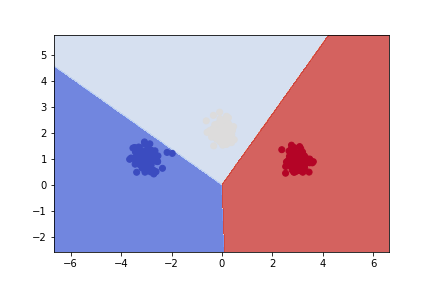
\includegraphics[width=\textwidth]{onevsall.png}\\
			\caption{One vs all classifier result} 
			\label{onevsall} 
		\end{figure}
		
		\pagebreak
		
		%%%%%%%%%%%%%%%%%%%%%%%%%%%%%%%%%%%%%%%%%%%%%%%%%%%%%%%%
		%6 .1.2
		%%%%%%%%%%%%%%%%%%%%%%%%%%%%%%%%%%%%%%%%%%%%%%%%%%%%%%%%
		\pagebreak
		\item {[}Optional{]} Normalize the vectors corresponding to each of the
		linear SVM classifiers so that they have unit norm. Evaluate the results
		and plot the decision regions for these normalized vectors.
		
		%%%%%%%%%%%%%%%%%%%%%%%%%%%%%%%%%%%%%%%%%%%%%%%%%%%%%%%%
		%6 .1.2 Answer
		%%%%%%%%%%%%%%%%%%%%%%%%%%%%%%%%%%%%%%%%%%%%%%%%%%%%%%%%
		Since we force the coefficients are force to have norm 1, we enforced a type of regularization. Our hypothesis space become smaller. Thus the results model became worse.
		\begin{figure}[ht]
			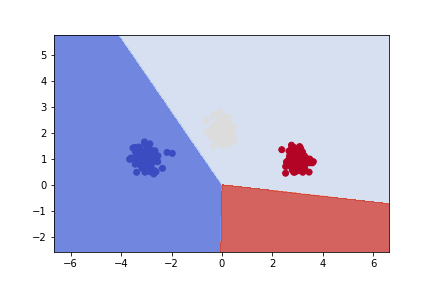
\includegraphics[width=\textwidth]{onevsall_normalized.png}\\
			\caption{One vs all classifier result with normalized weight} 
			\label{onevsall_norm} 
		\end{figure}
		\pagebreak
		
		
		\item {[}Optional{]} You may notice that every time you run the cell that
		fits the models and plots the decision regions, you get slightly different
		results. This is more pronounced when $C$ is larger, e.g. $C=200$.
		Investigate and propose an explanation for this. You may use any means
		necessary, including google searching and asking other people (just
		like in real life). {[}It's generally good to investigate things that
		look odd \textendash{} you'll almost always learn something, and sometimes
		you'll uncover a more serious underlying problem.{]}
	\end{enumerate}
	
	\pagebreak
	
	%%%%%%%%%%%%%%%%%%%%%%%%%%%%%%%%%%%%%%%%%%%%%%%%%%%%%%%%
	%6 .2 
	%%%%%%%%%%%%%%%%%%%%%%%%%%%%%%%%%%%%%%%%%%%%%%%%%%%%%%%%
	\subsection{Multiclass SVM}
	
	In this question, we will implement stochastic subgradient descent
	for the linear multiclass SVM described in lecture and in this problem
	set. We will use the class-sensitive feature mapping approach with
	the ``multivector construction'', as described in our \href{https://davidrosenberg.github.io/mlcourse/Lectures/7a.multiclass.pdf\#page=27}{multiclass classification lecture}
	and in SSBD Section 17.2.1. 
	\begin{enumerate}
		\item Complete the skeleton code for multiclass SVM. Following the multiclass
		SVM implementation, we have included another block of test code. Make
		sure to include the results from these tests in your assignment, along
		with your code. 
	\end{enumerate}
	%%%%%%%%%%%%%%%%%%%%%%%%%%%%%%%%%%%%%%%%%%%%%%%%%%%%%%%%
	%6 .2 Answer
	%%%%%%%%%%%%%%%%%%%%%%%%%%%%%%%%%%%%%%%%%%%%%%%%%%%%%%%%
	\begin{minted}{python}
	def zeroOne(y,a) :
	'''
	Computes the zero-one loss.
	@param y: output class
	@param a: predicted class
	@return 1 if different, 0 if same
	'''
	return int(y != a)
	
	def featureMap(X,y,num_classes) :
	'''
	Computes the class-sensitive features.
	@param X: array-like, shape = [n_samples,n_inFeatures] or [n_inFeatures,], input features for input data
	@param y: a target class (in range 0,..,num_classes-1)
	@return array-like, shape = [n_samples,n_outFeatures], the class sensitive features for class y
	'''
	#The following line handles X being a 1d-array or a 2d-array
	num_samples, num_inFeatures = (1,X.shape[0]) if len(X.shape) == 1 else (X.shape[0],X.shape[1])
	#your code goes here, and replaces following return
	#Applying multivector construction
	#Step 1: construct zero vectors of dimension num_samples*num_inFeatures
	num_outFeatures = num_classes*num_inFeatures
	output_X = np.zeros(num_samples*num_outFeatures).reshape(num_samples,num_outFeatures)
	#Create a method for num_samples == 1
	if num_samples == 1:
	feature_mapped = np.zeros(num_outFeatures)
	feature_mapped[y*num_inFeatures:(y+1)*num_inFeatures]=X
	return feature_mapped
	for idx,sample in enumerate(X):
	yi = y[idx]
	feature_mapped = np.zeros(num_outFeatures)
	feature_mapped[yi*num_inFeatures:(yi+1)*num_inFeatures]=sample
	output_X[idx,:] = feature_mapped
	return output_X
	
	def sgd(X, y, num_outFeatures, subgd, eta = 0.1, T = 10000):
	'''
	Runs subgradient descent, and outputs resulting parameter vector.
	@param X: array-like, shape = [n_samples,n_features], input training data 
	@param y: array-like, shape = [n_samples,], class labels
	@param num_outFeatures: number of class-sensitive features
	@param subgd: function taking x,y and giving subgradient of objective
	@param eta: learning rate for SGD
	@param T: maximum number of iterations
	@return: vector of weights
	'''
	num_samples = X.shape[0]
	#your code goes here and replaces following return statement
	w = np.zeros(num_outFeatures)
	# The following version is my first version of SGD but it kinds of fail.
	#     for t in range(T):
	#         pos = np.random.choice(num_samples,num_samples,replace=False)
	#         X = X[pos]
	#         y = y[pos]
	#         if t%1000==0:
	#             print('epoch:%s'%(t))
	#         for i,xi in enumerate(X):
	#             sg = subgd(xi,y[i],w)
	#             #print("sg:%s"%(sg))
	#             w = w - eta*sg
	#             #print("w:%s"%(w))
	#     return w
	# Following SSBD 17.2 p198
	avg_w = np.zeros(num_outFeatures)
	for t in range (T):
	pos = np.random.randint(300)
	x_sample = X[pos]
	y_sample = y[pos]
	vt = subgd(x_sample,y_sample,w) # using both version of subgradient works
	w -= eta*vt
	avg_w += w
	return avg_w/T
	
	
	
	class MulticlassSVM(BaseEstimator, ClassifierMixin):
	'''
	Implements a Multiclass SVM estimator.
	'''
	def __init__(self, num_outFeatures, lam=1.0, num_classes=3, Delta=zeroOne, Psi=featureMap):       
	'''
	Creates a MulticlassSVM estimator.
	@param num_outFeatures: number of class-sensitive features produced by Psi
	@param lam: l2 regularization parameter
	@param num_classes: number of classes (assumed numbered 0,..,num_classes-1)
	@param Delta: class-sensitive loss function taking two arguments (i.e., target margin)
	@param Psi: class-sensitive feature map taking two arguments
	'''
	self.num_outFeatures = num_outFeatures
	self.lam = lam
	self.num_classes = num_classes
	self.Delta = Delta
	self.Psi = lambda X,y : Psi(X,y,num_classes)
	self.fitted = False
	
	def subgradient(self,x,y,w):
	'''
	Computes the subgradient at a given data point x,y
	@param x: sample input
	@param y: sample class
	@param w: parameter vector
	@return returns subgradient vector at given x,y,w
	'''
	#Your code goes here and replaces the following return statement
	#Generalized hinge loss refered to hw5 3.2
	yi = y 
	#here y_prime is equivalent to y in 3.2 in problem set
	hxy = [self.Delta(yi,y_prime)+w.dot(self.Psi(x,y_prime))-w.dot(self.Psi(x,y))\
	for y_prime in range(self.num_classes)]
	yhat = np.where(hxy == max(hxy))[0][0]
	return 2*self.lam*w.T+self.Psi(x,yhat)-self.Psi(x,y)
	# Subgradient version from SSBD 17.2 page 198
	#return self.Psi(x,yhat)-self.Psi(x,y) 
	def fit(self,X,y,eta=0.1,T=10000):
	'''
	Fits multiclass SVM
	@param X: array-like, shape = [num_samples,num_inFeatures], input data
	@param y: array-like, shape = [num_samples,], input classes
	@param eta: learning rate for SGD
	@param T: maximum number of iterations
	@return returns self
	'''
	self.coef_ = sgd(X,y,self.num_outFeatures,self.subgradient,eta,T)
	self.fitted = True
	return self
	
	def decision_function(self, X):
	'''
	Returns the score on each input for each class. Assumes
	that fit has been called.
	@param X : array-like, shape = [n_samples, n_inFeatures]
	@return array-like, shape = [n_samples, n_classes] giving scores for each sample,class pairing
	'''
	if not self.fitted:
	raise RuntimeError("You must train classifer before predicting data.")
	
	#Your code goes here and replaces following return statement
	#Simon's Note: Please refer to hw5 2.2.1 for decision function
	#Question: Possibly using yhat definition in 3.3?
	hxy = np.zeros(len(X)*self.num_classes).reshape(len(X),self.num_classes)
	for i,xi in enumerate(X):
	hxy[i,:] = [self.coef_.dot(self.Psi(xi,yi)) for yi in range(self.num_classes)]
	return hxy
	
	def predict(self, X):
	'''
	Predict the class with the highest score.
	@param X: array-like, shape = [n_samples, n_inFeatures], input data to predict
	@return array-like, shape = [n_samples,], class labels predicted for each data point
	'''
	
	#Your code goes here and replaces following return statement
	def getmaxpos(arr1d):
	return np.where(arr1d==max(arr1d))[0][0]
	decision_mat = self.decision_function(X)
	return np.apply_along_axis(arr=decision_mat,axis=1,func1d=getmaxpos)
	\end{minted}
	\textbf{Results}
	\begin{figure}[ht]
		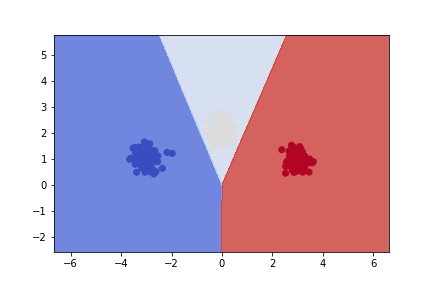
\includegraphics[width=\textwidth]{multisvm.png}\\
		\caption{Multi-class SVM classification results} 
		\label{onevsall_norm} 
	\end{figure}
	
	\pagebreak
	\section{{[}Optional{]} Audio Classification}
	
	In this problem, we will work on the urban sound dataset \href{https://serv.cusp.nyu.edu/projects/urbansounddataset/urbansound8k.html}{URBANSOUND8K}
	from the Center for Urban Science and Progress (CUSP) at NYU. We will
	first extract features from raw audio data using the \href{https://github.com/librosa/librosa}{LibROSA}
	package, and then we will train multiclass classifiers to classify
	the sounds into 10 sound classes. URBANSOUND8K dataset contains 8732
	labeled sound excerpts. For this problem, you may use the file UrbanSound8K.csv
	to randomly sample 2000 examples for training and 2000 examples for
	validation.
	\begin{enumerate}
		%%%%%%%%%%%%%%%%%%%%%%%%%%%%%%%%%%%%%%%%%%%%%%%%%%%%%%%%
		%7.1 
		%%%%%%%%%%%%%%%%%%%%%%%%%%%%%%%%%%%%%%%%%%%%%%%%%%%%%%%%
		
		\item In LibROSA, there are many functions for visualizing audio waves and
		spectra, such as display.waveplot() and display.specshow(). Load a
		random audio file from each class as a floating point time series
		with librosa.load(), and plot their waves and \href{https://librosa.github.io/librosa/generated/librosa.display.specshow.html}{linear-frequency power spectrogram}.
		If you are interested, you can also play the audio in the notebook
		with functions display() and Audio() in IPython.display. 
		%%%%%%%%%%%%%%%%%%%%%%%%%%%%%%%%%%%%%%%%%%%%%%%%%%%%%%%%
		%7.1 Answer
		%%%%%%%%%%%%%%%%%%%%%%%%%%%%%%%%%%%%%%%%%%%%%%%%%%%%%%%%
		\textbf{Use the following codes to plot}
		\begin{minted}{python}
		#Extract sound metadata
		info = pd.read_csv('../../datasets/UrbanSound8K/metadata/UrbanSound8K.csv')
		#store class samples to plot
		samples_path = []
		#Create a training set
		filenames_train =[]
		folds_train = []
		classIDs_train = []
		def getpath(directory,fold_num,filename):
		intermediate = os.path.join(directory,'fold')+str(fold_num)
		return(os.path.join(intermediate,filename))
		for classid in range(10):
		subset = info[info['classID']==classid].iloc[:200]
		filenames_train+=subset['slice_file_name'].values.tolist()
		classIDs_train+=subset['classID'].values.tolist()
		folds_train+=subset['fold'].values.tolist()
		samples_path.append(getpath(directory='../../datasets/UrbanSound8K/audio/',fold_num=folds_train[-1],filename=filenames_train[-1]))
		filepaths_train = [os.path.join('../../datasets/UrbanSound8K/audio/fold'+str(folds_train[idx]),filenames_train[idx])\
		for idx in range(len(filenames_train))]
		
		#X_train = [lb.core.load(filepath)[0] for filepath in filepaths_train]
		# #Create a validation set
		# filenames_valid =[]
		# classIDs_valid = []
		# for classid in range(10):
		#     subset = info[info['classID']==classid]
		#     filenames_valid.append(subset.iloc[200:400]['slice_file_name'].values.astype('str'))
		#     classIDs_valid.append(subset.iloc[200:400]['classID'].values)
		
		plt.figure(figsize=(20,10))
		for idx,path in enumerate(samples_path):
		y = lb.core.load(path)[0]
		D = lb.amplitude_to_db(lb.stft(y), ref=np.max)
		plt.subplot(2,5,idx+1)
		if idx in [0,5]:
		display.specshow(D,y_axis='linear')
		else:
		display.specshow(D)
		plt.title('Sample Class: %s'%(idx))
		\end{minted}
		\begin{figure}[ht]
			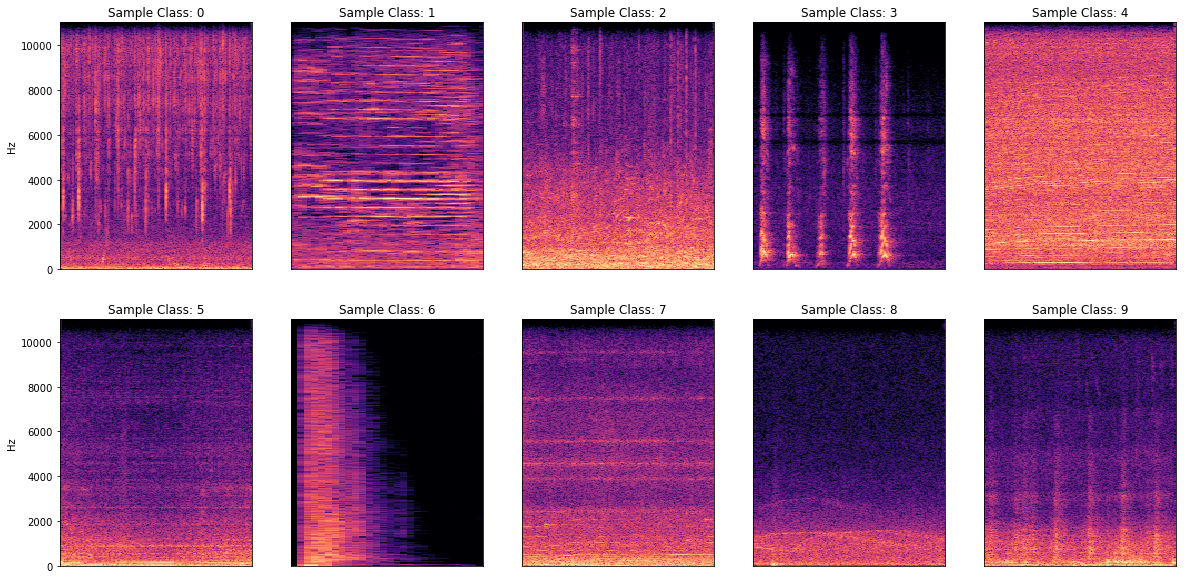
\includegraphics[width=\textwidth]{spectrum.png}\\
			\caption{Spectrum} 
			\label{onevsall_norm} 
		\end{figure}
		\pagebreak
		\item \href{https://en.wikipedia.org/wiki/Mel-frequency_cepstrum}{Mel-frequency cepstral coefficients (MFCC)}
		are a commonly used feature for sound processing. We will use MFCC
		and its first and second differences (like discrete derivatives) as
		our features for classfication. First, use function feature.mfcc()
		from LibROSA to extract MFCC features from each audio sample. (The
		first MFCC coefficient is typically discarded in sound analysis, but
		you do not need to. You can test whether this helps in the optional
		problem below.) Next, use function feature.delta() to calculate the
		first and second differences of MFCC. Finally, combine these features
		and normalize each feature to zero mean and unit variance.
		\pagebreak
		\item Train a linear multiclass SVM on your 2000 example training set. Evaluate
		your results on the validation set in terms of 0/1 error and generate
		a confusion table. Compare the results to a one-vs-all classifier
		using a binary linear SVM as the base classifier. For each model,
		may use your code from the previous problem, or you may use another
		implementation (e.g. from sklearn). 
		\pagebreak
		\item {[}More Optional{]} Compare results to any other multiclass classification
		methods of your choice. 
		\pagebreak
		\item {[}More Optional{]} Try different feature sets and see how they affect
		performance.
	\end{enumerate}
	
\end{document}
